\documentclass{beamer}
%\documentclass[handout]{beamer}
\usepackage{pgfpages}
\mode<handout>{%
  \pgfpagesuselayout{2 on 1}[a4paper]
  \setbeameroption{show notes}
}

\usepackage{microtype}
\usepackage{kotex}
\usepackage{amssymb, amsmath, mathtools}


%%%%%%%%%%%%%%%%%%%%%%%%%%%%%%%%%%%%%%%%%%%%%%%%%%%%%%%%%%%%%%%%%%%%%%%%%%%%%%%
%%%%%%%%%%%%%%%%%%%%%%%%%%%%%%%%% Beamer setup %%%%%%%%%%%%%%%%%%%%%%%%%%%%%%%%
%%%%%%%%%%%%%%%%%%%%%%%%%%%%%%%%%%%%%%%%%%%%%%%%%%%%%%%%%%%%%%%%%%%%%%%%%%%%%%%
\usetheme[
  numbering = fraction,
  progressbar = frametitle,
  sectionpage = progressbar,
  subsectionpage = progressbar,
]{metropolis}

\useoutertheme{infolines}
\usecolortheme{rose}

\setbeamertemplate{itemize item}[square]
\setbeamertemplate{itemize subitem}[triangle]
\setbeamertemplate{itemize subsubitem}[circle]
% \setbeamertemplate{mini frames}{}

\setbeamercolor{background~canvas}{bg=white}

\titlegraphic{%
  \begin{tikzpicture}[overlay, remember picture]
    \node at (current page.35) [xshift=-3em, yshift=-1.3em] {
      
\includegraphics[width=3em]{img/snulife-symbol.png}
    };
  \end{tikzpicture}%
}


%%%%%%%%%%%%%%%%%%%%%%%%%%%%%%%%%%%%%%%%%%%%%%%%%%%%%%%%%%%%%%%%%%%%%%%%%%%%%%%
%%%%%%%%%%%%%%%%%%%%%%%%%%%%%%%%% Font setup %%%%%%%%%%%%%%%%%%%%%%%%%%%%%%%%%%
%%%%%%%%%%%%%%%%%%%%%%%%%%%%%%%%%%%%%%%%%%%%%%%%%%%%%%%%%%%%%%%%%%%%%%%%%%%%%%%

% Works for pdfLaTeX, XeLaTeX, and LuaLaTeX
\usepackage{libertine}

% Math/Mono font setup
\ExplSyntaxOn
\bool_if:nTF { \sys_if_engine_xetex_p: || \sys_if_engine_luatex_p: }
  {
    \usepackage[
      math-style=ISO,
      warnings-off={mathtools-colon, mathtools-overbracket},
    ]{unicode-math}
    \setmathfont{LibertinusMath-Regular.otf}[Scale = MatchUppercase]
    \setmathfont{Garamond-Math.otf}[
      Scale = MatchUppercase,
      range = {\Coloneq}
    ]

    \setmonofont{MonaspaceArgon}[
      Extension = .otf,
      UprightFont = *-Regular,
      BoldFont = *-Bold,
      ItalicFont = *-Italic,
      BoldItalicFont = *-BoldItalic,
      Scale=MatchLowercase,
    ]

    \setmainhangulfont{Noto Serif CJK KR}[
      FakeSlant = 0.2,
      UprightFont = *-Regular,
      BoldFont = *-Bold,
    ]
    \setsanshangulfont[BoldFont={* Bold}]{KoPubWorldDotum_Pro}
    \setmonohangulfont{D2Coding}
  }
  {
    \usepackage[libertine]{newtxmath}
    \usepackage{inconsolata}
  }
\ExplSyntaxOff


%%%%%%%%%%%%%%%%%%%%%%%%%%%%%%%%%%%%%%%%%%%%%%%%%%%%%%%%%%%%%%%%%%%%%%%%%%%%%%%
%%%%%%%%%%%%%%%%%%%%%%%%%%%%%%%% Presentations %%%%%%%%%%%%%%%%%%%%%%%%%%%%%%%%
%%%%%%%%%%%%%%%%%%%%%%%%%%%%%%%%%%%%%%%%%%%%%%%%%%%%%%%%%%%%%%%%%%%%%%%%%%%%%%%


\usepackage{minted}
\usemintedstyle{solarized-light}
\definecolor{solarized-bg}{RGB}{253,246,227}
\ExplSyntaxOn
\NewDocumentCommand { \NewMinted } { m }
  {
    \clist_map_inline:nn { #1 }
      {
        \newminted { ##1 }
          {
            bgcolor = solarized-bg,
            baselinestretch = 1.2,
            stripall = true,
            breaklines = true,
            fontsize = \tiny,
            autogobble = true,
          }
      }
  }
\ExplSyntaxOff
\NewMinted{ocaml, py, swift, c, cpp, rs, js, ts}

\usepackage{listings}
\lstset{
  basicstyle = \ttfamily,
  mathescape,
}

% \usepackage{codehigh}
% \let\fverb\fakeverb

\usepackage{ebproofx}
\ebproofxset{right label template = \textsc{\smaller[2]\inserttext}}
\newcommand*{\longcenter}[1]{\[\makebox[\textwidth][c]{#1}\]}

\usepackage{simplebnf}
\SetBNFLayout{
  column{1} = {font = \sffamily},
  column{2} = {mode = dmath},
  column{4} = {mode = dmath},
}


% Korean-English, e.g., \alt{메모리 재활용}{garbage collection}
% \alt*을 통해 찾아보기에 추가, \alt는 단순히 한영 병기
% <>안에는 참조할 다른 개념 제시
\ExplSyntaxOn

\NewDocumentCommand { \myindex } { s m m }
  {
    \IfBooleanTF {#1}
      { \index{#2!#3|textbf}\index{#3!#2|textbf} }
      { \index{#2!#3}\index{#3!#2} }
  }

\NewDocumentCommand { \Alt } { s m O{#2} d<> m O{#5} d<> }
  {
    #2\,{\color{gray}\smaller\textit{#5}}\hspace{.06667em}
    \IfBooleanT {#1}
      {
        \myindex{#3}{#6}

        \IfNoValueTF {#4}
          {
            \IfNoValueF {#7}
              { % See English
                \index{#6|see{#7}}
              }
          }
          {
            \IfNoValueTF {#7}
              { % See Korean
                \index{#3|see{#4}}
              }
              { % See both
                \index{#3|see{#4}}\index{#6|see{#7}}
              }
          }
      }
  }
\ExplSyntaxOff


%%%%%%%%%%%%%%%%%%%%%%%%%%%%%%%%%%%%%%%%%%%%%%%%%%%%%%%%%%%%%%%%%%%%%%%%%%%%%%%
%%%%%%%%%%%%%%%%%%%%%%%%%%%%%%%% Miscellaneous %%%%%%%%%%%%%%%%%%%%%%%%%%%%%%%%
%%%%%%%%%%%%%%%%%%%%%%%%%%%%%%%%%%%%%%%%%%%%%%%%%%%%%%%%%%%%%%%%%%%%%%%%%%%%%%%

% C++ logo
\usepackage{relsize}
\def\cplus{\raisebox{.4ex}{\relsize{-3}{\texttt{+}}}}
\def\C++{C\nolinebreak\hspace{-.081em}\cplus\nolinebreak\hspace{-0.02em}\cplus}


\usetikzlibrary{calc,decorations.pathmorphing,shapes}
\newcounter{sarrow}
\newcommand\xrsquigarrow[1]{%
  \stepcounter{sarrow}%
  \mathrel{%
    \begin{tikzpicture}[
      > = stealth,
      baseline = {($(current bounding box.south) + (0,-0.5ex)$)}
    ]
      \node[inner sep = .5ex] (\thesarrow) {$\scriptstyle #1$};
      \path[
        draw,
        <-,
        semithick,
        decorate,
        decoration = {
          zigzag,
          amplitude = 1pt,
          segment length = 1.2mm,
          pre = lineto,
          pre length = 4pt
        }
      ] (\thesarrow.south east) -- (\thesarrow.south west);
    \end{tikzpicture}%
  }%
}



\usepackage{hyperref}


%% Default info
\title{타입으로 안전하게 프로그래밍하기}
\institute{SNULife 개발팀}
\date{2024년 1월 13일}
\author{이재호}

\begin{document}
\maketitle

\begin{frame}[c, fragile]
  \frametitle{목차}
  \tableofcontents[subsectionstyle=hide]
\end{frame}

\section{타입 시스템이란?}
\begin{frame}[c, fragile]
  \frametitle{``자유로운'' 언어의 숙명}

  \only<1>{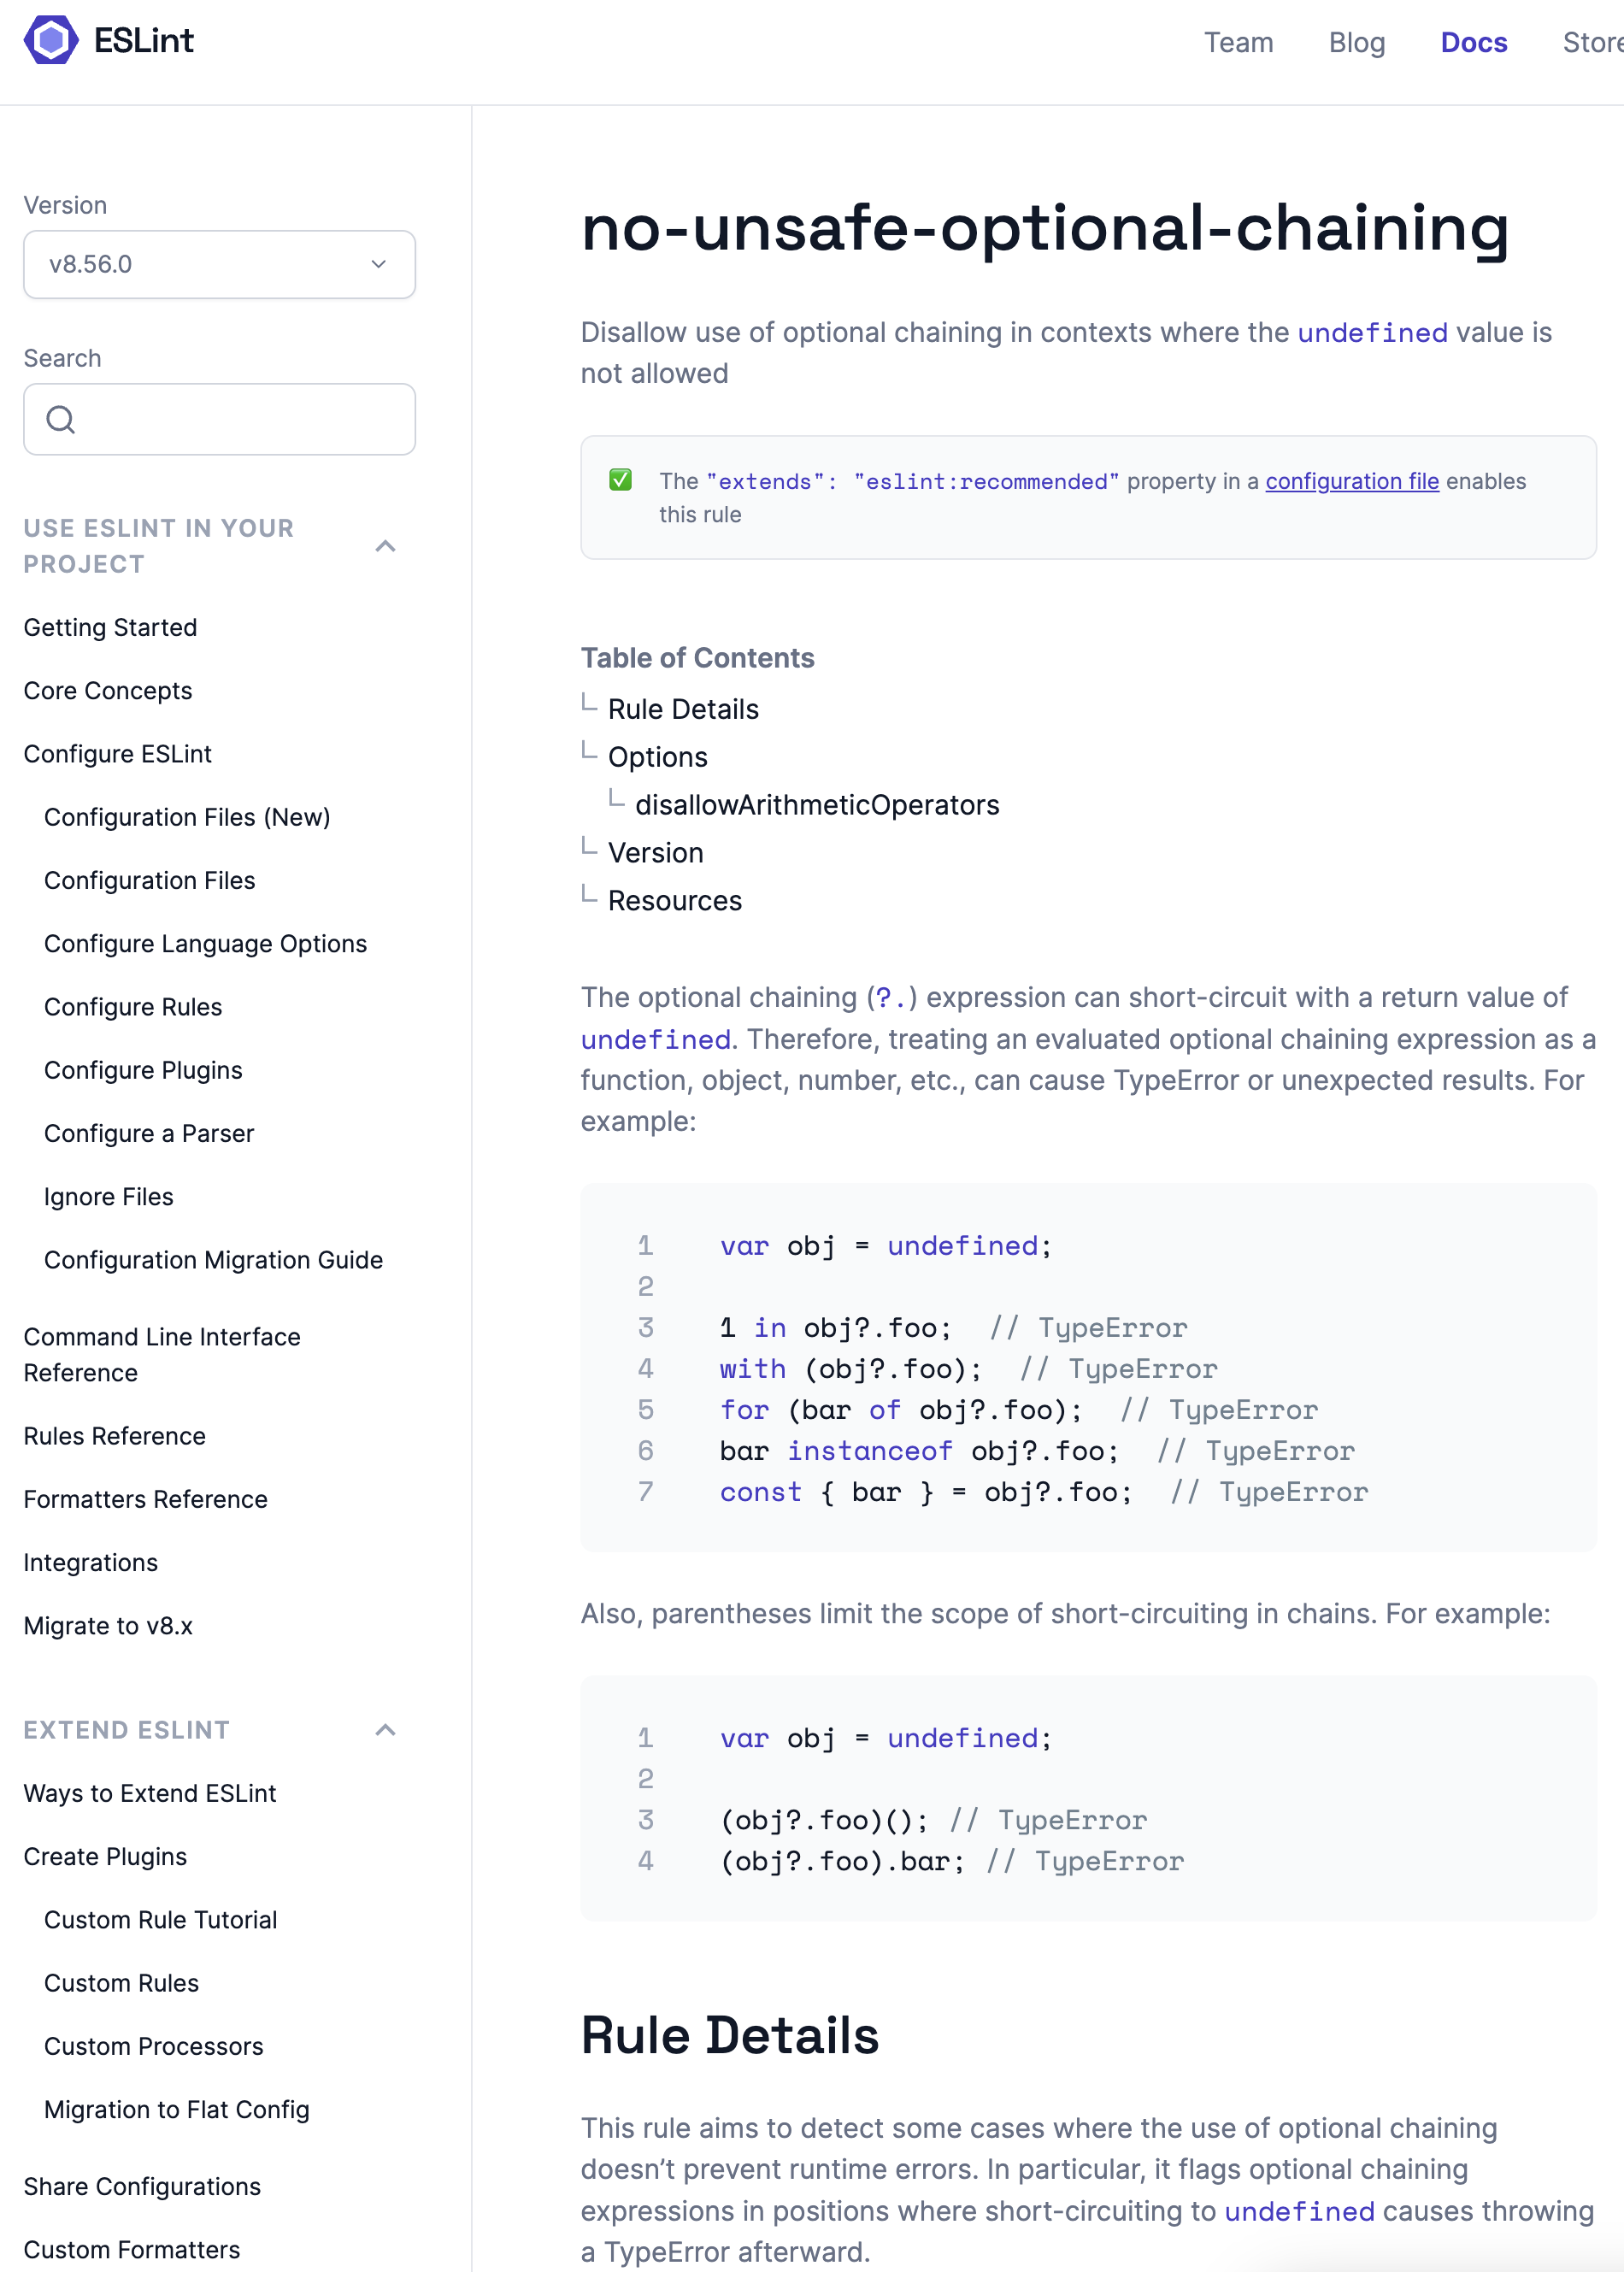
\includegraphics[width=\linewidth]{img/es-lint.png}}

  \begin{onlyenv}<2>
    \begin{quote}
      This rule aims to detect some cases where the use of optional chaining doesn’t prevent runtime errors.
      In particular, it flags optional chaining expressions in positions where short-circuiting to \texttt{undefined} causes throwing a TypeError afterward.
    \end{quote}%
    \begin{jscode}
      /*eslint no-unsafe-optional-chaining: "error"*/
      (obj?.foo)();
      (obj?.foo).bar;
      (foo?.()).bar;
      (foo?.()).bar();
    \end{jscode}
  \end{onlyenv}

  \only<3>{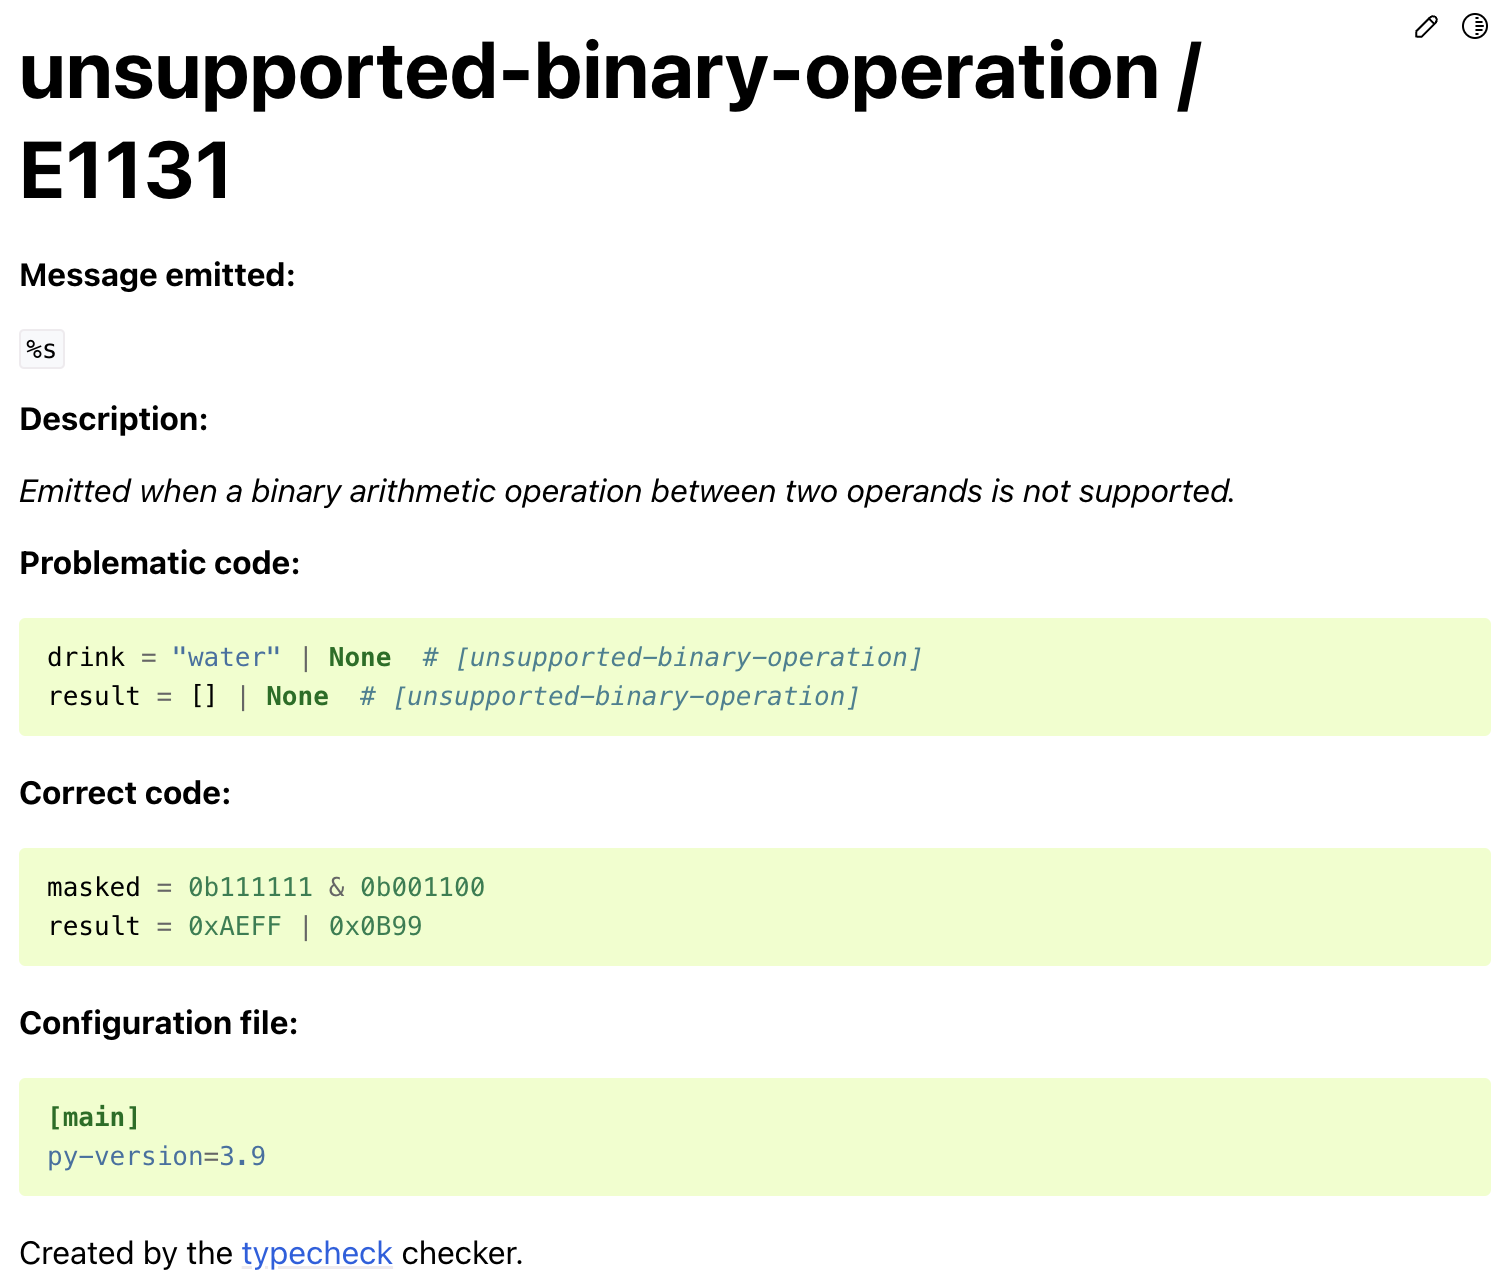
\includegraphics[width=\linewidth]{img/pylint.png}}
\end{frame}

\begin{frame}[c, fragile]
  \frametitle{동적 타입과 정적 타입}

  동적 타입 시스템은 사실 ``타입 시스템''이 아닌 실행 중 타입 태그 검사
  {\footnotesize\begin{description}
    \item[동적 타입 언어] \Alt*{파이썬}{Python}, \Alt*{자바스크립트}{JavaScript}, \Alt*{스킴}{Scheme}, \Alt*{라켓}{Racket}, \Alt*{루아}{Lua}, \Alt*{루비}{Ruby}, \Alt*{펄}{Perl}, \Alt*{라쿠}{Raku}, \ldots
    \item[정적 타입 언어] \Alt*{스위프트}{Swift}, \Alt*{코틀린}{Kotlin}, \Alt*{러스트}{Rust}, \Alt*{오캐멀}{OCaml}, \Alt*{하스켈}{Haskell}, \Alt*{리스크립트}{ReScript}, \Alt*{엚}{Elm}, C, \C++, \Alt*{자바}{Java}, \ldots
  \end{description}}

  \begin{onlyenv}<2>
    \begin{pycode}
Python 3.11.4 (main, Jul  4 2023, 19:38:47) [Clang 14.0.3 (clang-1403.0.22.14.1)] on darwin
Type "help", "copyright", "credits" or "license" for more information.
>>> def poison():
...     "hello" + 42
...
>>> poison()
Traceback (most recent call last):
  File "<stdin>", line 1, in <module>
  File "<stdin>", line 2, in poison
TypeError: can only concatenate str (not "int") to str
    \end{pycode}
  \end{onlyenv}
  
  \begin{onlyenv}<3>
    \begin{swiftcode}
  Welcome to Apple Swift version 5.9.2 (swiftlang-5.9.2.2.56 clang-1500.1.0.2.5).
Type :help for assistance.
  1> func poison() {
  2.     "hello" + 42
  3. }
error: repl.swift:2:13: error: binary operator '+' cannot be applied to operands of type 'String' and 'Int'
    "hello" + 42
    ~~~~~~~ ^ ~~

repl.swift:2:13: note: overloads for '+' exist with these partially matching parameter lists: (Int, Int), (String, String)
    "hello" + 42
            ^
    \end{swiftcode}
  \end{onlyenv}

  \begin{onlyenv}<4>
    \begin{ocamlcode}
OCaml version 5.1.0
Enter #help;; for help.

# let poison () = "hello" + 42;;
Error: This expression has type string but an expression was expected of type
         int
    \end{ocamlcode}
  \end{onlyenv}

  \begin{onlyenv}<5>
    \begin{jscode}
Welcome to Node.js v20.10.0.
Type ".help" for more information.
> function poison() {
... "hello" + 42
... }
undefined
> poison()
undefined
> "hello" + 42
'hello42'
    \end{jscode}
    ???
  \end{onlyenv}
  \only<6>{\begin{center}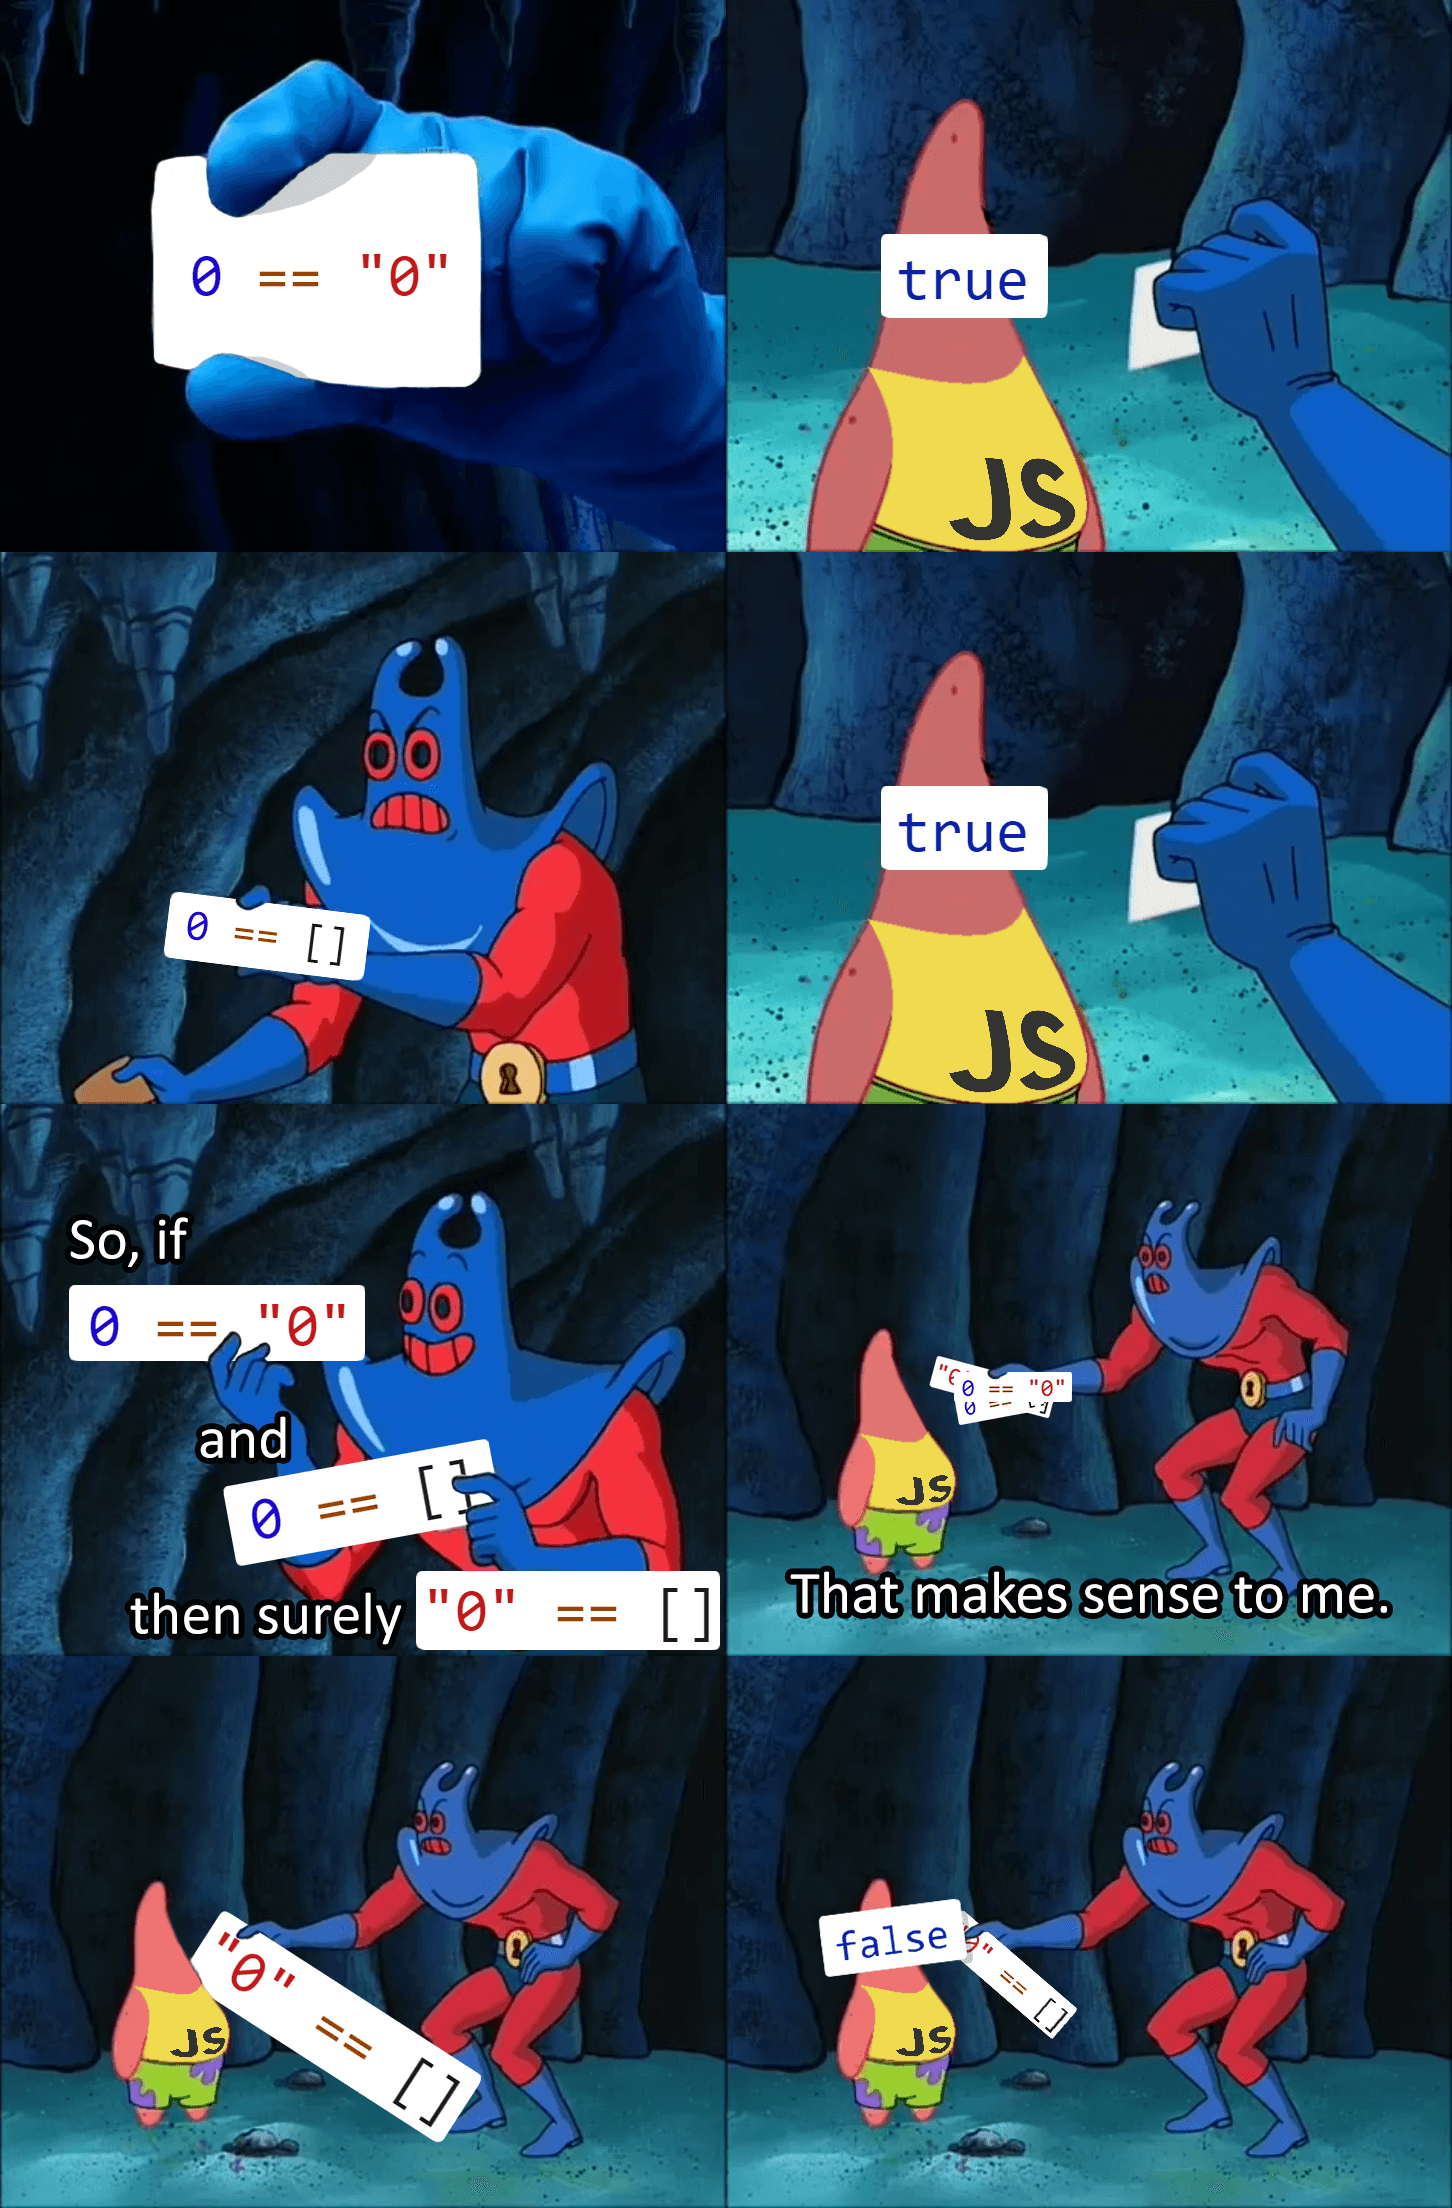
\includegraphics[width=0.27\linewidth]{img/js-meme.png}\end{center}}
\end{frame}

\begin{frame}[c, fragile]
  \frametitle{타입 시스템}

  타입 시스템은 \textbf{실행 전}에 프로그램이 \textbf{잘} 실행될 수 있는지를 \textbf{겉모습}으로 검사하는 방법

  \begin{description}
    \item[실행 전에]<2-> 오류를 \Alt*{안전하게}{sound}\ 잡아냄
    \item[잘]<3-> 만족해야 하는 성질을 타입 시스템에 녹여낼 수 있고, 실행 중에 어긋나는 일이 없음
    \item[겉모습]<4->, 즉 문법적으로 검사를 할 수 있음
  \end{description}
\end{frame}


\section{타입 시스템의 장점}
\subsection{\Alt*{안전성}{Soundness}}
\begin{frame}[c, fragile]
  \frametitle{잘 타입된 프로그램은 잘못되지 않는다}
  % TODO: better quote
  ``Well-type programs cannot go wrong'' \smaller{--- Robin Milner, in \textit{A Theory of Type Polymorphism in Programming} (1978)}

  (\Alt*{안전한}{Sound}) 타입 시스템을 갖춘 언어에서는 실행 중 타입 에러가 발생하지 않는다!
\end{frame}


\begin{frame}[c, fragile]
  \frametitle{안전한 타입 시스템이란?}

  안전성은 실행 중에 ``잘'' 만족해야 하는 성질이 어긋나지 않는 것을 의미
  \begin{itemize}
    \item 그 성질은 언어마다 다름
    \item 통상적인 타입 시스템은 실행 과정에서 계산된 값이 실제로 타입된 것과 일치하는지를 의미
  \end{itemize}
  \pause 안전한 타입 시스템이 중요한 이유
  \begin{itemize}
    \item 타입을 통해 원하는 성질을 표현할 수 있다면, 실제로 값이 그 성질을 만족한다고 신뢰할 수 있음
      \pause\begin{itemize}
        \item 리스트가 비어있지 않다는 성질을 \textbf{보장}하는 타입?
      \end{itemize}
    \pause\item 이러한 성질이 충분히 강력하다면, 테스트나 다른 프로그램 검증 기법 없이도 확신할 수 있음
      \pause\begin{itemize}
        \item 이것의 극단은 \Alt*{콕}{Coq}, \Alt*{아그다}{Agda}, \Alt*{린}{Lean}\ 등과 같은 \Alt*{값에 기댄 타입 언어}{dependently typed language}
      \end{itemize}
  \end{itemize}
\end{frame}
\note[itemize]{
  \item 비어있지 않는 리스트 타입은 뒤에 일반화된 합과 곱 타입을 사용해 보여줄 예정
}


\begin{frame}[c, fragile]
  \frametitle{\Alt*{조금씩 타입 붙이기}{Gradual typing}}

  동적인 언어에 타입 시스템을 도입하는 방법
  \begin{itemize}
    \item 안전성에 방점을 두지 않음
    \item 버그를 잡는데 도움
  \end{itemize}
  \pause\begin{description}
    \item[자바스크립트] 타입스크립트, \Alt*{플로우}{Flow}
    \item[파이썬] \Alt*{마이파이}{MyPy}, \Alt*{파이어}{Pyre}, \Alt*{파이라이트}{Pyright}, \Alt*{파이타이프}{Pytype}
    \item[루비] \Alt*{소르베}{Sorbet}
    \item[라켓] \Alt*{타입 라켓}{Typed Racket}
    \item[라쿠] 언어 자체에 내장
  \end{description}
\end{frame}


\begin{frame}[c, fragile]
  \frametitle{안전하지 않은 타입 시스템: 타입스크립트}

  타입스크립트는 안전하지 않은 타입 시스템

  \begin{center}
    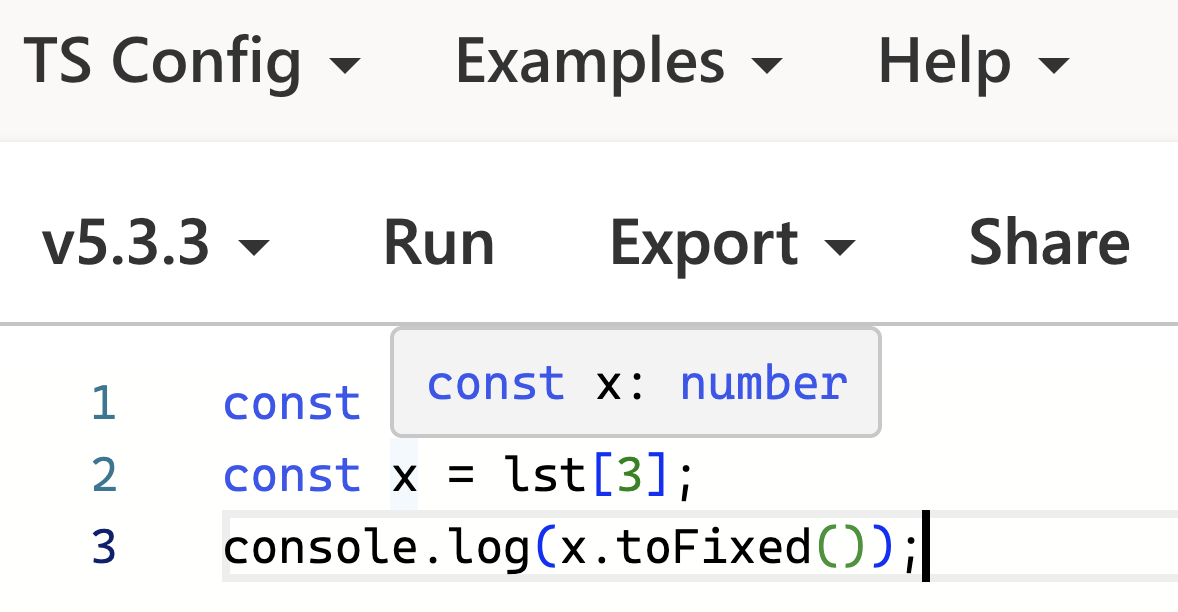
\includegraphics[width=0.6\linewidth]{img/ts-unsound.png}
  \end{center}

  \begin{tscode}
Welcome to Node.js v20.10.0.
Type ".help" for more information.
> const lst = [3, 1, 4];
undefined
> const x = lst[3];  // static type is number but runtime type is undefined.
undefined
> console.log(x.toFixed());
Uncaught TypeError: Cannot read properties of undefined (reading 'toFixed')
  \end{tscode}
\end{frame}
\note[itemize]{
  \item 타입 시스템을 염두하지 않고 만든 언어에 안전한 타입 시스템을 도입하는 것은 어려움
  \item 이러한 언어에서는 타입 검증이 어려운 상용구를 지향하기도 함
}

\begin{frame}[c, fragile]
  \frametitle{안전하게 조금씩 타입 붙이기}

  타입스크립트는 안전하지 않은 타입 시스템

  \begin{center}
    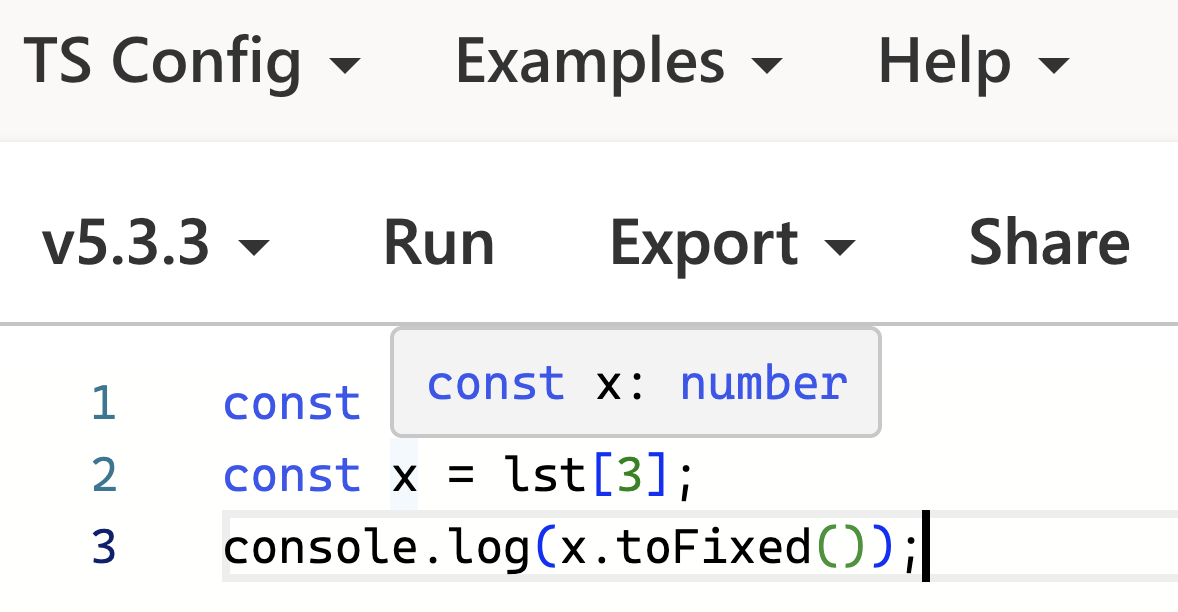
\includegraphics[width=0.6\linewidth]{img/ts-unsound.png}
  \end{center}

  \begin{tscode}
Welcome to Node.js v20.10.0.
Type ".help" for more information.
> const lst = [3, 1, 4];
undefined
> const x = lst[3];  // static type is number but runtime type is undefined.
undefined
> console.log(x.toFixed());
Uncaught TypeError: Cannot read properties of undefined (reading 'toFixed')
  \end{tscode}
\end{frame}


\begin{frame}[c, fragile]
  \frametitle{안전하지 않은 타입 시스템: 수동 메모리 관리}

  수동 메모리 관리를 지원하는 언어는 안전한 타입 시스템을 만들기 굉장히 어려움

  \begin{ccode}
    int toxic(void)
    {
            int *x = malloc(sizeof(int));
            *x = 42;
            int *y = x;
            free(x);
            float *z = malloc(sizeof(float));
            *z = 3.141592f;
            return *y + 1;
    }
  \end{ccode}

  \begin{onlyenv}<2>
     \Alt*{메모리 재활용}{Garbage collection}은 필수적(이었음)
     \begin{itemize}
         \item 러스트는 소유권과 빌려주기의 개념을 사용해 문제를 우회
     \end{itemize}
  \end{onlyenv}
\end{frame}


\subsection{성능 향상}
\begin{frame}[c, fragile]
  \frametitle{미루지 말고 미리미리}

  정적 타입 시스템은 실행 전에 타입을 검사하기 때문에,
  \begin{itemize}
    \item 실행 중에 타입 검사를 할 필요가 없고
    \item 효율적으로 값을 메모리에 담을 수 있음
  \end{itemize}

  \pause\begin{pycode}
Python 3.11.4 (main, Jul  4 2023, 19:38:47) [Clang 14.0.3 (clang-1403.0.22.14.1)] on darwin
Type "help", "copyright", "credits" or "license" for more information.
>>> 42 + "foo"
Traceback (most recent call last):
  File "<stdin>", line 1, in <module>
TypeError: unsupported operand type(s) for +: 'int' and 'str'
  \end{pycode}
\end{frame}


\subsection{관계 표현}
\begin{frame}[c, fragile]
  \frametitle{간증: \Alt*{서로 맞물려 돌아가는}{mutually recursive}\ 구조}

  \begin{onlyenv}<1>
    \tiny\url{https://easyword.kr}
    \vskip-1.4em\begin{center}
      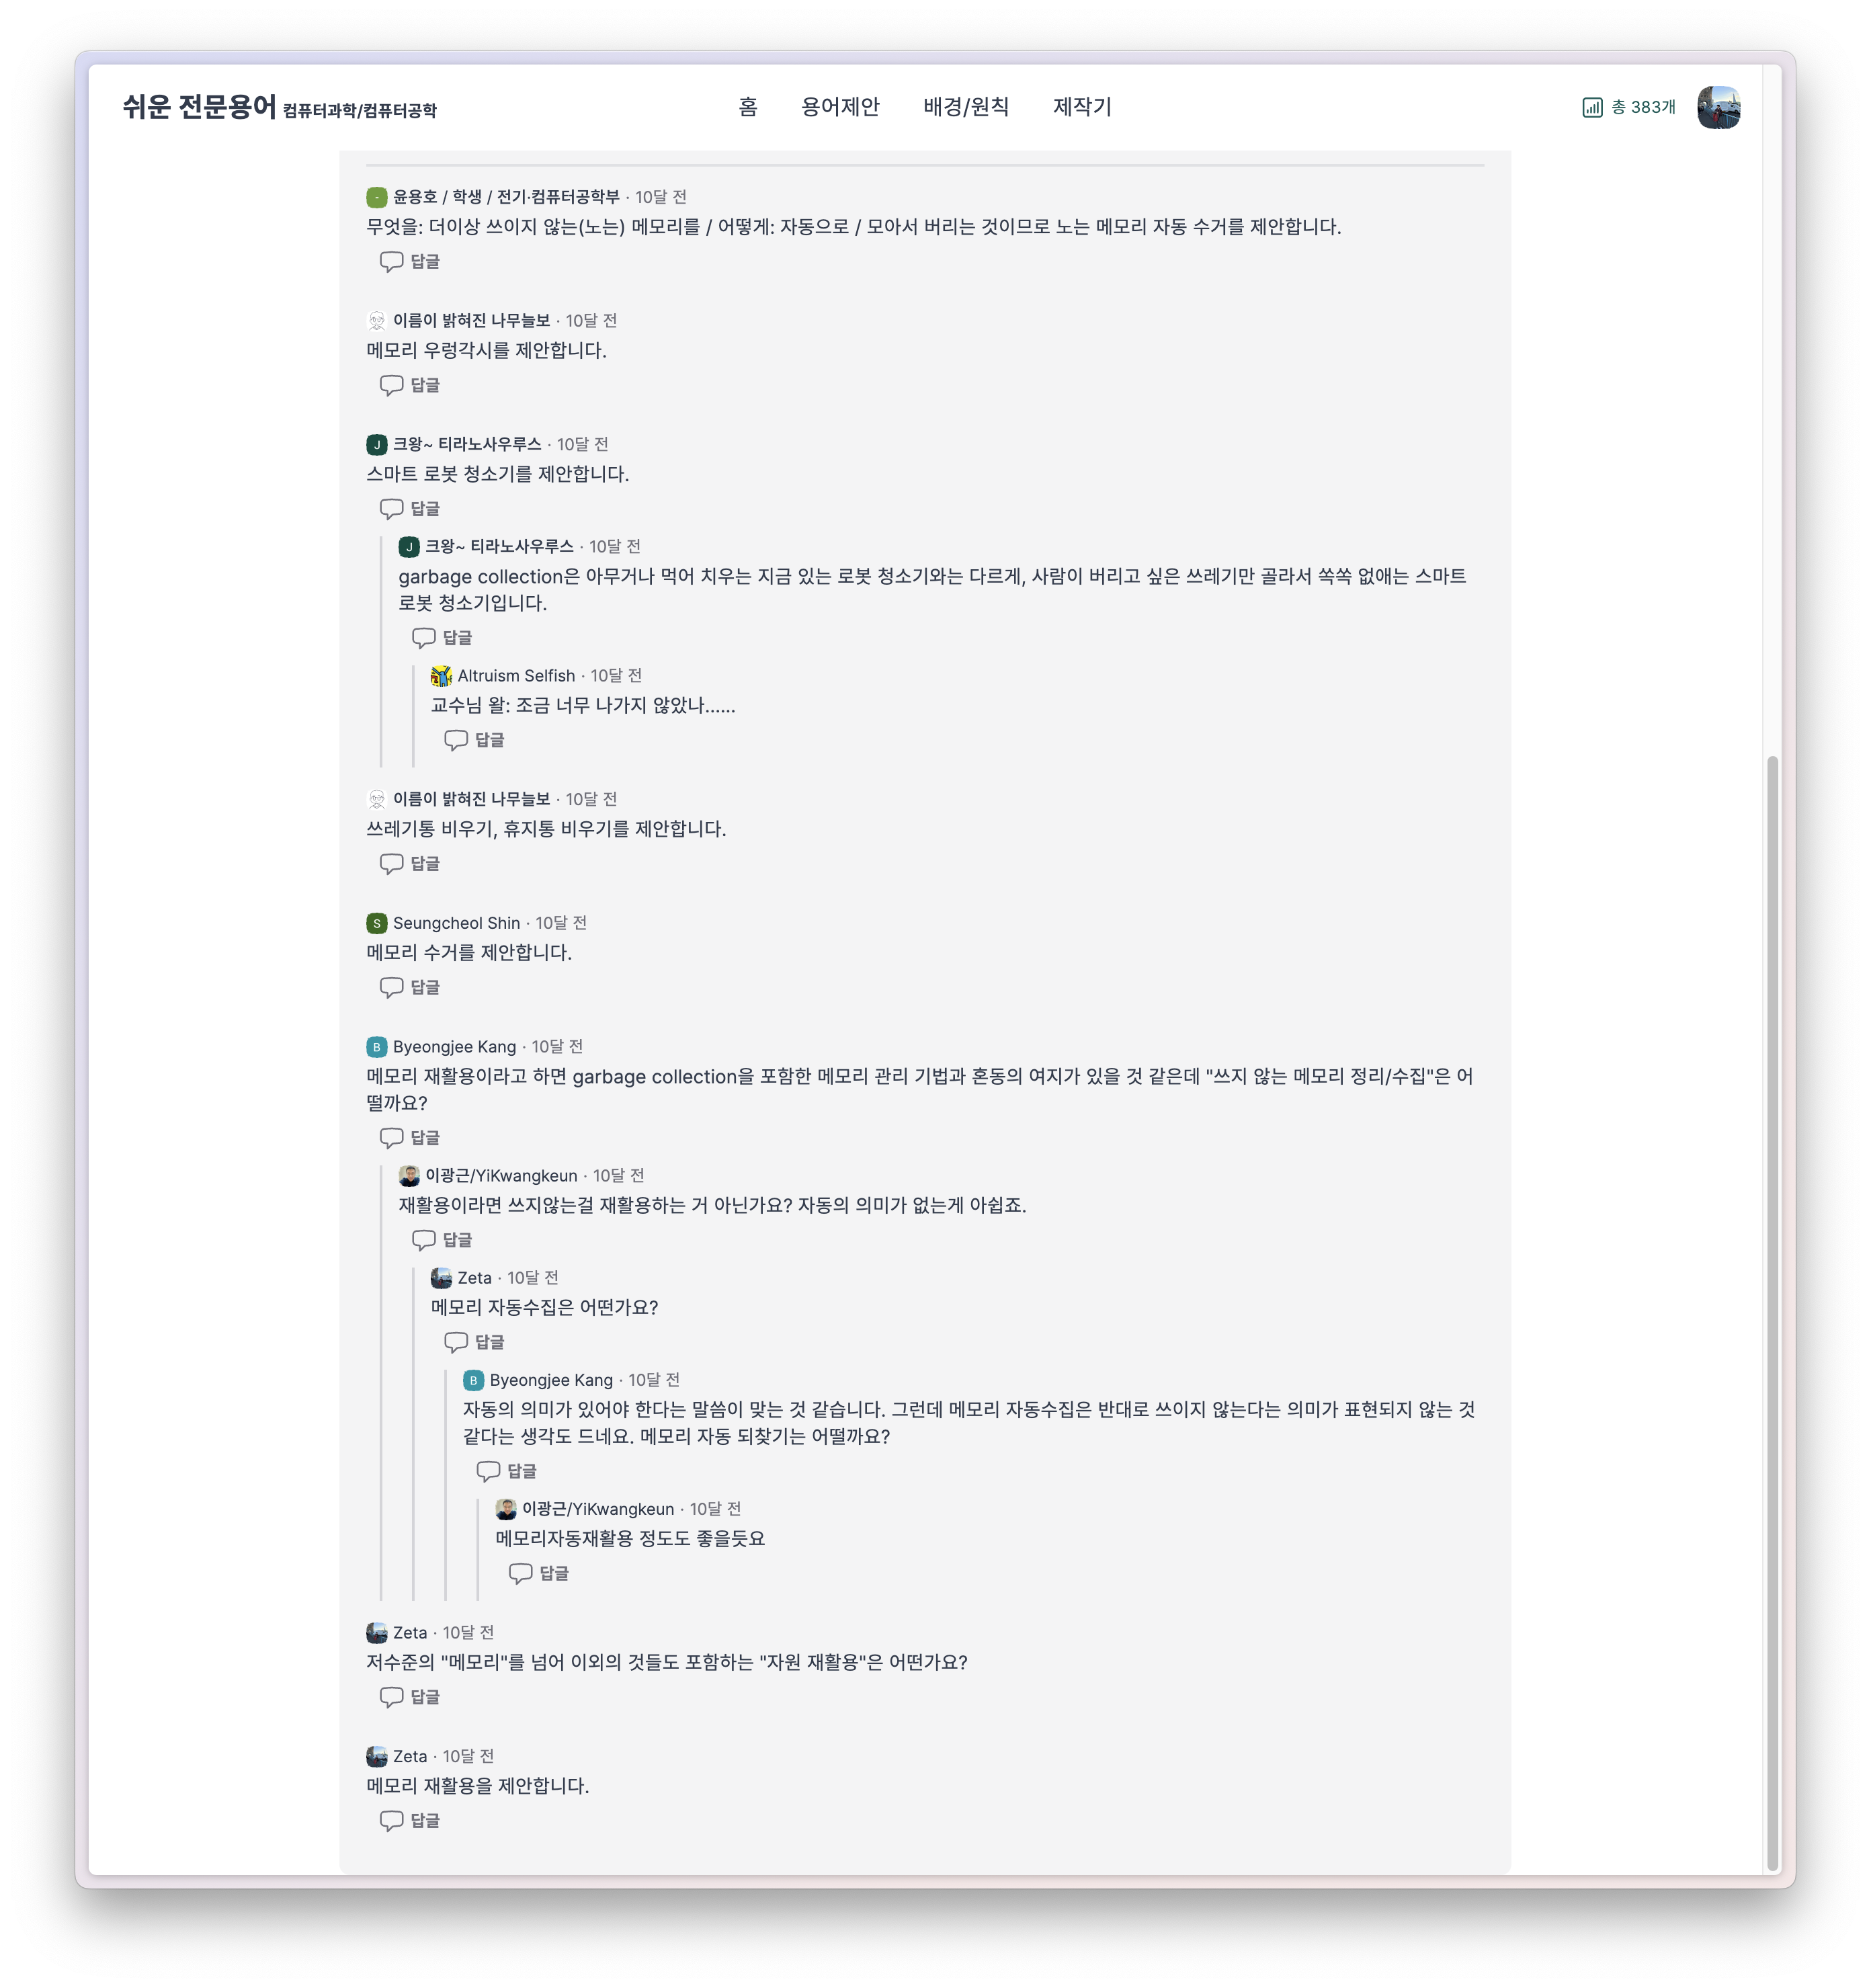
\includegraphics[width=0.6\linewidth]{img/easyword.png}
    \end{center}
  \end{onlyenv}

  \begin{onlyenv}<2>
    \mbox{\small\url{https://github.com/Zeta611/eko/blob/main/src/Comment.res}}\footnote{영구 링크: \href{https://github.com/Zeta611/eko/blob/9d140e8b578030b99a0965719be7aa8fd7f18899/src/Comment.res}{\texttt{https://github.com/Zeta611/eko/...}}}
    \vskip-1em
    \begin{ocamlcode}
  // Firestore comment entity
  @deriving({abstract: light})
  type t = {
    @optional id: string,
    content: string,
    user: string,
    timestamp: Firebase.Timestamp.t,
    parent: string,
  }
  type rec node = {
    comment: t,
    mutable parent: option<node>,
    mutable children: list<node>,
  }
  let rec countDescendents = children => {
    switch children {
    | list{} => 0
    | list{{children}, ...tl} => 1 + countDescendents(children) + countDescendents(tl)
    }
  }
    \end{ocamlcode}
  \end{onlyenv}
\end{frame}

\begin{frame}[c, fragile]
  \frametitle{맛보기: 여러 종류의 다형성}

  \scriptsize\begin{description}
    \item[매개변수 다형성] \texttt{CollapsibleView}가 받아들이는 \texttt{State}, \texttt{Control}, \texttt{Collapsible} 타입
    \item[타입 적응 다형성] \texttt{State} 타입은 \texttt{Togglable}의 모양(스위프트에서는 \Alt*{프로토콜}{protocol}이라고 부름)을, \texttt{Control}과 \texttt{Collapsible} 타입은 \texttt{View}의 모양을 가짐
      \begin{itemize}
        \item \texttt{CollapsibleView}는 \texttt{View}의 모양을 가짐
      \end{itemize}
    \item[아래 타입 다형성] 아래 코드에는 드러나지 않았지만, \texttt{Togglable} 타입은 \texttt{Equatable}의 아래 타입
  \end{description}
  \href{https://github.com/snulife/snulife-gp-ios-2/blob/cded38ba6f728bf5429520424a8326ac4cc23a1b/GP/Views/CollapsibleView.swift#L11}{\texttt{CollapsibleView.swift}}
  \begin{swiftcode}
struct CollapsibleView<State: Togglable, Control: View, Collapsible: View>: View {
    @Binding var globalState: State
    let state: State
    let control: () -> Control
    let collapsible: () -> Collapsible
    @FocusState private var foo: Bool
    private let val = false

    var body: some View { ... }

    init( ... ) { ... }
}
  \end{swiftcode}
\end{frame}


\section{타입 시스템과 다형성}
\subsection{간단한 타입 시스템}
\begin{frame}[c, fragile]
  \frametitle{\Alt*{람다 계산법}{Lambda Calculus}}

  람다 계산법은 계산의 원리를 연구하기 위해 만들어진 수학적 모델 (Alonzo Church, 1920대)
  \begin{itemize}
    \item 그런데 프로그래밍 언어를 설명하는데 효과적이라는 것이 밝혀짐! (Peter Landin, 1960대)
  \end{itemize}

  \pause\begin{pycode}
Python 3.11.4 (main, Jul  4 2023, 19:38:47) [Clang 14.0.3 (clang-1403.0.22.14.1)] on darwin
Type "help", "copyright", "credits" or "license" for more information.
>>> fact = lambda n: 1 if n == 0 else n * fact(n - 1)
>>> fact(10)
3628800
  \end{pycode}
  \pause
  \begin{center}
    fact = $\lambda$ n. if n = 0 then 1 else n * fact(n - 1)
  \end{center}
\end{frame}

\begin{frame}[c, fragile]
  \frametitle{람다 계산법의 \Alt*{문법 구조}{syntax}와 \Alt*{실행 의미 구조}{operational semantics}}

  \begin{minipage}[t]{0.49\linewidth}
    문법 구조
    \begin{center}
      \begin{bnf}
        t : 항 ::=
        | x : 변수
        | \lambda x.t : 함수
        | t\ t : 적용
        ;;
        v : 값 ::=
        | \lambda x.t : 함수 값
      \end{bnf}
    \end{center}
  \end{minipage}
  \begin{minipage}[t]{0.49\linewidth}
    실행 의미 구조\hfill\fbox{$t \rightsquigarrow t'$}
    \begin{center}
      \begin{InfRule}{E-App1}
        \hypo{t_1 \rightsquigarrow t_1'}
        \infer1{t_1\ t_2 \rightsquigarrow t_1'\ t_2}
      \end{InfRule}
      \begin{InfRule}{E-App2}
        \hypo{t_2 \rightsquigarrow t_2'}
        \infer1{v_1\ t_2 \rightsquigarrow v_1\ t_2'}
      \end{InfRule}
      \begin{InfRule}{E-AppAbs}
        \infer0{(\lambda x.t_{12})\ v_2 \rightsquigarrow [x \mapsto v_2]t_{12}}
      \end{InfRule}
    \end{center}
  \end{minipage}
  \pause\[\begin{tblr}{rl}
    & (\lambda x.\lambda y.x)\ \underline{((\lambda x.x)\ a)}\ b \\
    \xrsquigarrow{\textsc{E-App2, E-AppAbs}} & \underline{(\lambda x.\lambda y.x)\ a}\ b \\
    \xrsquigarrow{\textsc{E-App1, E-AppAbs}} & \underline{(\lambda y.a)\ b} \\
    \xrsquigarrow{\textsc{E-App1}} & a
  \end{tblr}\]
\end{frame}


\begin{frame}[c, fragile]
  \frametitle{\Alt*{간단한 타입을 가진 람다 계산법}{Simply Typed Lambda Calculus, STLC}}

  \begin{minipage}[t]{0.49\linewidth}
    문법 구조
    \begin{center}
      \def\typecolon{{:}}
      \begin{bnf}
        t : 항 ::=
        | x : 변수
        | \lambda x \typecolon \tau.t : 함수
        | t\ t : 적용
        ;;
        v : 값 ::=
        | \lambda x \typecolon \tau .t : 함수 값
        ;;
        \tau : 타입 ::=
        | \tau \to \tau : 함수 타입
        ;;
        \Gamma : 환경 ::=
        | \varnothing : 빈 환경
        | \Gamma, x \mathrel{\typecolon} \tau : 변수 타입 정의
      \end{bnf}
    \end{center}
  \end{minipage}
  \begin{minipage}[t]{0.49\linewidth}
    타입 규칙\hfill\fbox{$\Gamma \vdash t : \tau$}
    \begin{center}
      \begin{InfRule}{T-Var}
        \hypo{x : \tau \in \Gamma}
        \infer1{\Gamma \vdash x : \tau}
      \end{InfRule}
      \begin{InfRule}{T-Abs}
        \hypo{\Gamma, x : \tau_1 \vdash t_2 : \tau_2}
        \infer1{\Gamma \vdash \lambda x {:} \tau_1.t_2 : \tau_1 \to \tau_2}
      \end{InfRule}
      \begin{InfRule}{T-App}
        \hypo{\Gamma \vdash t_1 : \tau_{11} \to \tau_{12}}
        \hypo{\Gamma \vdash t_2 : \tau_{11}}
        \infer{1,1}{\Gamma \vdash t_1\ t_2 : \tau_{12}}
      \end{InfRule}
    \end{center}
  \end{minipage}
\end{frame}


\begin{frame}[c, fragile]
  \frametitle{타입 규칙 예시}

  새로운 불리언 항 \texttt{true}, \texttt{false}를 추가하고, 불리언 타입 \texttt{Bool}을 추가:
  \begin{center}
    \begin{InfRule}{T-True}
      \infer0{\Gamma \vdash \texttt{true} : \texttt{Bool}}
    \end{InfRule}
    \begin{InfRule}{T-False}
      \infer0{\Gamma \vdash \texttt{false} : \texttt{Bool}}
    \end{InfRule}
  \end{center}

  \begin{prooftree*}
    \hypo{\texttt{x} : \texttt{Bool} \in \texttt{x} : \texttt{Bool}}
    \infer1[T-Var]{\texttt{x} : \texttt{Bool} \vdash \texttt{x} : \texttt{Bool}}
    \infer1[T-Abs]{\vdash \lambda \texttt{x}{:}\texttt{Bool}.\texttt{x} : \texttt{Bool} \to \texttt{Bool}}
    \infer0[T-True]{\vdash \texttt{true} : \texttt{Bool}}
    \infer2[T-App]{\vdash (\lambda \texttt{x}{:}\texttt{Bool}.\texttt{x})\ \texttt{true} : \texttt{Bool}}
  \end{prooftree*}
\end{frame}


\subsection{\Alt*{매개변수 다형성}{Parametric polymorphism}}
\begin{frame}[c, fragile]
  \frametitle{매개변수 다형성의 동기}

  인터넷에서 데이터를 가져오는 함수 \verb/fetch/를 만들어보자!
  \begin{itemize}
    \pause\item 그런데 데이터의 타입마다 다른 함수를 만들어야 하나?
  \end{itemize}
  \pause 타입에 상관없이 동작하는 \Alt*{일반적인}{generic} 함수를 만들고 싶다!
  \begin{swiftcode}
  func fetch<T>(
      _ type: T.Type,
      router: Router,
      accessToken: String? = nil
  ) async throws -> T where T: Decodable {
      logger.debug("fetch(\(type), router: \(router.path), accessToken: \(accessToken ?? "nil")")
      let request = try generateRequest(router: router, accessToken: accessToken)
      let (data, response) = try await session.data(for: request)
  ... }
  \end{swiftcode}
  대충:
  \[
    \texttt{fetch} : \forall \texttt{T}. \texttt{T.Type} \to \texttt{Router} \to \texttt{String?} \to \texttt{T}
  \]
\end{frame}

\begin{frame}[c, fragile]
  \frametitle{시스템 F}

  \scriptsize
  \begin{minipage}[t]{0.49\linewidth}
    문법 구조
    \begin{center}
      \def\typecolon{{:}}
      \begin{bnf}
        t : 항 ::=
        | x : 변수
        | \lambda x \typecolon \tau.t : 함수
        | t\ t : 적용
        | \Lambda X.t : 타입 함수
        | t [\tau] : 타입 적용
        ;;
        v : 값 ::=
        | \lambda x \typecolon \tau .t : 함수 값
        | \Lambda X.t : 타입 함수 값
        ;;
        \tau : 타입 ::=
        | X : 타입 변수
        | \tau \to \tau : 함수 타입
        | \forall X.\tau : 보편 타입
        ;;
        \Gamma : 환경 ::=
        | \varnothing : 빈 환경
        | \Gamma, x \mathrel{\typecolon} \tau : 변수 타입 정의
        | \Gamma, X : 타입 변수 정의
      \end{bnf}
    \end{center}
  \end{minipage}
  \begin{onlyenv}<1>
    \begin{minipage}[t]{0.49\linewidth}
      실행 의미 구조\hfill\fbox{$t \rightsquigarrow t'$}
      \begin{center}
        \begin{InfRule}{E-App1}
          \hypo{t_1 \rightsquigarrow t_1'}
          \infer1{t_1\ t_2 \rightsquigarrow t_1'\ t_2}
        \end{InfRule}
        \begin{InfRule}{E-App2}
          \hypo{t_2 \rightsquigarrow t_2'}
          \infer1{v_1\ t_2 \rightsquigarrow v_1\ t_2'}
        \end{InfRule}
        \begin{InfRule}{E-AppAbs}
          \infer0{(\lambda x.t_{12})\ v_2 \rightsquigarrow [x \mapsto v_2]t_{12}}
        \end{InfRule}
        \begin{InfRule}{E-TApp}
          \hypo{t_1 \rightsquigarrow t_1'}
          \infer1{t_1[\tau_2] \rightsquigarrow t_1'[\tau_2]}
        \end{InfRule}
        \begin{InfRule}{E-TAppTAbs}
          \infer0{(\Lambda X.t_{12})[\tau_2] \rightsquigarrow [X \mapsto \tau_2]t_{12}}
        \end{InfRule}
      \end{center}
    \end{minipage}
  \end{onlyenv}
  \begin{onlyenv}<2>
    \begin{minipage}[t]{0.49\linewidth}
      타입 규칙\hfill\fbox{$\Gamma \vdash t : \tau$}
      \begin{center}
        \begin{InfRule}{T-Var}
          \hypo{x : \tau \in \Gamma}
          \infer1{\Gamma \vdash x : \tau}
        \end{InfRule}
        \begin{InfRule}{T-Abs}
          \hypo{\Gamma, x : \tau_1 \vdash t_2 : \tau_2}
          \infer1{\Gamma \vdash \lambda x{:}\tau_1.t_2 : \tau_1 \to \tau_2}
        \end{InfRule}
        \begin{InfRule}{T-App}
          \hypo{\Gamma \vdash t_1 : \tau_{11} \to \tau_{12}}
          \hypo{\Gamma \vdash t_2 : \tau_{11}}
          \infer{1,1}{\Gamma \vdash t_1\ t_2 : \tau_{12}}
        \end{InfRule}
        \begin{InfRule}{T-TAbs}
          \hypo{\Gamma, X \vdash t_2 : \tau_2}
          \infer1{\Gamma \vdash \Lambda X.t_2 : \forall X.\tau_2}
        \end{InfRule}
        \begin{InfRule}{T-TApp}
          \hypo{\Gamma \vdash t_1 : \forall X. \tau_{12}}
          \infer1{\Gamma \vdash t_1[\tau_2] : [X \mapsto \tau_2]\tau_{12}}
        \end{InfRule}
      \end{center}
    \end{minipage}
  \end{onlyenv}
\end{frame}


\begin{frame}[c, fragile]
  \frametitle{시스템 F의 예시}

\begin{lstlisting}
double = $\Lambda$X. $\lambda$f: X $\to$ X. $\lambda$x: X. f (f x)
> double : $\forall$X. (X $\to$ X) $\to$ X $\to$ X

doubleInt = double [Int]
> doubleInt : (Int $\to$ Int) $\to$ Int $\to$ Int

doubleIntArrowInt = double [Int $\to$ Int]
> doubleIntArrowInt : ((Int $\to$ Int) $\to$ Int $\to$ Int)
                      $\to$ (Int $\to$ Int) $\to$ Int $\to$ Int

quadruple = $\Lambda$X. double [X $\to$ X] (double [X])
> quadruple : $\forall$X. (X $\to$ X) $\to$ X $\to$ X
\end{lstlisting}
\end{frame}


\begin{frame}[c, fragile]
  \frametitle{\Alt*{let 다형성}{let-polymorphism}}
  \tiny
  \begin{ocamlcode}
OCaml version 5.1.0
Enter #help;; for help.

# let double f a = f (f a);;
val double : ('a -> 'a) -> 'a -> 'a = <fun>
# double ((+) 1) 1;;
- : int = 3
# double ((+.) 1.) 1.;;
- : float = 3.
# let quadruple = double double;;
val quadruple : ('_weak1 -> '_weak1) -> '_weak1 -> '_weak1 = <fun>
# quadruple ((+) 1) 1;;
- : int = 5
# quadruple ((+.) 1.) 1.;;
Error: This expression has type float -> float
       but an expression was expected of type int -> int
       Type float is not compatible with type int
# let quadruple a = double double a;;
val quadruple : ('a -> 'a) -> 'a -> 'a = <fun>
# quadruple ((+) 1) 1;;
- : int = 5
# quadruple ((+.) 1.) 1.;;
- : float = 5.
  \end{ocamlcode}
\end{frame}


\subsection{\Alt*{아래 타입 다형성}{Subtype polymorphism}}
\begin{frame}[c, fragile]
  \frametitle{\texttt{Self}의 기묘함}

  \begin{swiftcode}
Welcome to Apple Swift version 5.9.2 (swiftlang-5.9.2.2.56 clang-1500.1.0.2.5).
Type :help for assistance.
  1> class A {
  2.     let x: Int
  3.     func isEqual(to other: Self) -> Bool {
  4.         self.x == other.x
  5.     }
  6.     init(x: Int) {
  7.         self.x = x
  8.     }
  9. }
error: repl.swift:3:28: error: covariant 'Self' or 'Self?' can only appear as the type of a property, subscript or method result; did you mean 'A'?
    func isEqual(to other: Self) -> Bool {
                           ^~~~
                           A
  \end{swiftcode}

  \pause \verb/A/를 상속하는 클래스의 \verb/isEqual(to:)/가 이상하다!
\end{frame}


\begin{frame}[c, fragile]
  \frametitle{\Alt*{맞춰 변하기}{covariant}, \Alt*{거슬러 변하기}{contravariant}, \Alt*{안 변하기}{invariant}}

  같은 타입의 다른 값과 같은지 비교하는 함수를 만들자:
  \begin{ocamlcode}
OCaml version 5.1.0
Enter #help;; for help.
# type x = [ `X ];;
type x = [ `X ]
# type xy = [ `X | `Y ];;
type xy = [ `X | `Y ]
# let x : x = `X;;
val x : x = `X
# let x' = (x :> xy);;
val x' : xy = `X
# let l : x list = [`X; `X];;
val l : x list = [`X; `X]
# let l' = (l :> xy list);;
val l' : xy list = [`X; `X]
# let f : xy -> unit = function `X -> () | `Y -> ();;
val f : xy -> unit = <fun>
# let f' = (f :> x -> unit);;
val f' : x -> unit = <fun>
# let x : x ref = ref `X;;
val x : x ref = {contents = `X}
# let x' = (x :> xy ref);;
Error: Type x ref is not a subtype of xy ref
       The first variant type does not allow tag(s) `Y
  \end{ocamlcode}
\end{frame}


\begin{frame}[c, fragile]
  \frametitle{아래 타입 다형성}

  \tiny
  \begin{minipage}[t]{0.49\linewidth}
    문법 구조
    \begin{center}
      \def\typecolon{{:}}
      \begin{bnf}
        t : 항 ::=
        | x : 변수
        | \lambda x \typecolon \tau.t : 함수
        | t\ t : 적용
        ;;
        v : 값 ::=
        | \lambda x \typecolon \tau .t : 함수 값
        ;;
        \tau : 타입 ::=
        | \top : 최대 타입
        | \tau \to \tau : 함수 타입
        ;;
        \Gamma : 환경 ::=
        | \varnothing : 빈 환경
        | \Gamma, x \mathrel{\typecolon} \tau : 변수 타입 정의
      \end{bnf}
    \end{center}
    실행 의미 구조\hfill\fbox{$t \rightsquigarrow t'$}
    \begin{center}
      \begin{InfRule}{E-App1}
        \hypo{t_1 \rightsquigarrow t_1'}
        \infer1{t_1\ t_2 \rightsquigarrow t_1'\ t_2}
      \end{InfRule}
      \begin{InfRule}{E-App2}
        \hypo{t_2 \rightsquigarrow t_2'}
        \infer1{v_1\ t_2 \rightsquigarrow v_1\ t_2'}
      \end{InfRule}
      \begin{InfRule}{E-AppAbs}
        \infer0{(\lambda x.t_{12})\ v_2 \rightsquigarrow [x \mapsto v_2]t_{12}}
      \end{InfRule}
    \end{center}
  \end{minipage}
  \begin{minipage}[t]{0.49\linewidth}
    아래 타입 규칙\hfill\fbox{$\varsigma <: \tau$}
    \begin{center}
      \begin{InfRule}{S-Refl}
        \infer0{\varsigma <: \varsigma}
      \end{InfRule}
      \begin{InfRule}{S-Trans}
        \hypo{\varsigma <: \upsilon}
        \hypo{\upsilon <: \tau}
        \infer2{\varsigma <: \tau}
      \end{InfRule}
      \begin{InfRule}{S-Top}
        \infer0{\varsigma <: \top}
      \end{InfRule}
      \begin{InfRule}{S-Arrow}
        \hypo{\tau_1 <: \varsigma_1}
        \hypo{\varsigma_2 <: \tau_2}
        \infer2{\varsigma_1 \to \varsigma_2 <: \tau_1 \to \tau_2}
      \end{InfRule}
    \end{center}
    타입 규칙\hfill\fbox{$\Gamma \vdash t : \tau$}
    \begin{center}
      \begin{InfRule}{T-Var}
        \hypo{x : \tau \in \Gamma}
        \infer1{\Gamma \vdash x : \tau}
      \end{InfRule}
      \begin{InfRule}{T-Abs}
        \hypo{\Gamma, x : \tau_1 \vdash t_2 : \tau_2}
        \infer1{\Gamma \vdash \lambda x{:}\tau_1.t_2 : \tau_1 \to \tau_2}
      \end{InfRule}
      \begin{InfRule}{T-App}
        \hypo{\Gamma \vdash t_1 : \tau_{11} \to \tau_{12}}
        \hypo{\Gamma \vdash t_2 : \tau_{11}}
        \infer2{\Gamma \vdash t_1\ t_2 : \tau_{12}}
      \end{InfRule}
      \begin{InfRule}{T-Sub}
        \hypo{\Gamma \vdash t : \varsigma}
        \hypo{\varsigma <: \tau}
        \infer2{\Gamma \vdash t : \tau}
      \end{InfRule}
    \end{center}
  \end{minipage}
\end{frame}

\subsection{\Alt*{타입 적응 다형성}{Ad-hoc polymorphism}}
\begin{frame}[c, fragile]
  \frametitle{타입 적응 다형성}

  파이썬을 떠올려보면, \verb/+/ 연산자는 정수, 실수, 문자열, 리스트 등 다양한 타입에 대해 다양한 의미를 가짐
  \begin{itemize}
    \pause\item C를 떠올려보면, \verb/+/ 연산자를 문자열이나 배열에 대해 사용하는 것은 상상도 못함
    \pause\item \C++에서는 된다!
  \end{itemize}
  연산자 및 함수를 같은 이름으로 여러 벌 만드는 \Alt*{오버로딩}{overloading}
  \begin{cppcode}
class X
{
public:
    X& operator+=(const X& rhs) { /* ... */ return *this; }
    friend X operator+(X lhs, const X& rhs)
    {
        lhs += rhs;
        return lhs;
    }
};
  \end{cppcode}

\end{frame}


\section{타입 시스템 구멍내기}
\begin{frame}[c, fragile]
  \frametitle{강제로 타입 변환하기}

  대부분의 언어는 강제로 타입을 변환하는 기능을 제공
  \begin{itemize}
    \item 타입 변환 혹은 메모리 재해석
    \item \Alt*{FFI}{Foreign Function Interface}를 위해서 필요하기도 함
  \end{itemize}

  \begin{tscode}
> const a = 42 as string
<repl>.ts:4:11 - error TS2352: Conversion of type 'number' to type 'string' may be a mistake because neither type sufficiently overlaps with the other. If this was intentional, convert the expression to 'unknown' first.

4 const a = 42 as string
            ~~~~~~~~~~~~

> const a = 42 as unknown as string
undefined
  \end{tscode}
\end{frame}

\begin{frame}[c, fragile]
  \frametitle{스위프트의 \Alt*{불투명한 타입}{opaque type}}

  \begin{quotation}
Swift provides two ways to hide details about a value’s type: opaque types and boxed protocol types. Hiding type information is useful at boundaries between a module and code that calls into the module, because the underlying type of the return value can remain private.

A function or method that returns an opaque type hides its return value’s type information. Instead of providing a concrete type as the function’s return type, the return value is described in terms of the protocols it supports. Opaque types preserve type identity — \textbf{the compiler has access to the type information, but clients of the module don’t.}
  \end{quotation}
\hfill---\href{https://docs.swift.org/swift-book/documentation/the-swift-programming-language/opaquetypes/}{The Swift Programming Language, Opaque Types}
\end{frame}

\begin{frame}[c, fragile]
  \frametitle{조심스럽게 타입 변환하기}

  \begin{minipage}[t]{0.49\linewidth}
    ...도 문제다!
    \begin{swiftcode}
    protocol Color<T> {
      associatedtype T
      var red: T { get }
      var blue: T { get }
      func print(_: T) -> String
    }
    struct ColorInt: Color {
      let red = 0
      let blue = 1
      func print(_ x: Int) -> String {
        switch x {
        case 0: "red"
        case 1: "blue"
        default: ""
        }
      }
    }
    \end{swiftcode}
  \end{minipage}
  \begin{minipage}[t]{0.50\linewidth}
    \begin{swiftcode}
    struct ColorBool: Color {
      let red = true
      let blue = false
      func print(_ x: Bool) -> String {
        x ? "red" : "blue"
      }
    }
    func eqZero<T>(_ x: T) -> Bool {
      guard let x = x as? Int else { return false }
      return x == 0
    }
    let c1: some Color = ColorInt()
    let c2: some Color = ColorBool()
    print(c1.print(c1.red))  // "red"
    print(c2.print(c2.red))  // "red"
    print(eqZero(c1.red))  // true
    print(eqZero(c2.red))  // false
    \end{swiftcode}
  \end{minipage}
\end{frame}


\section{타입 시스템 100\%{} 활용하기}
\subsection{\Alt*{곱의 합 타입}{Algebraic Data Type, ADT}}
\begin{frame}[c, fragile]
  \frametitle{모든 경우 빠짐 없이 나타내기}

  \begin{minipage}[t]{0.49\linewidth}
    \begin{swiftcode}
  enum Router {
      case login(LoginParameters)
      case logout(LogoutParameters)
      case refresh(RefreshParameters)
      case me
      case timetableList
      case timetableRead(uuidString: String)
      /* ... */ }
  enum Method {
      case get([URLQueryItem])
      case post(Content, [URLQueryItem])
      case patch(Content, [URLQueryItem])
      case delete
      var name: String {
          switch self {
          case .get: return "GET"
          /* ... */ } } }
    \end{swiftcode}
  \end{minipage}
  \begin{minipage}[t]{0.49\linewidth}
    \begin{swiftcode}
    var method: Method {
        switch self {
        case let .login(loginParameters):
            guard let data = try? Self.jsonEncoder.encode(loginParameters) else {
                // ...
                return .post(.applicationJSON(nil), [])
            }
            return .post(.applicationJSON(data), [])
    /* ... */ } } }
    \end{swiftcode}
    \texttt{switch}가 모든 경우를 다 다루고 있음을 컴파일러가 검증
  \end{minipage}
\end{frame}


\begin{frame}[c, fragile]
  \frametitle{\Alt*{저예산 곱의 합 타입}{Poor man's ADT}}

    \begin{ccode}
/* https://github.com/Zeta611/polycalc/blob/main/src/term.h
 * Diagram of the representation for 2xy^2 + 5y + 9 using `TermNode`s
 *  hd   u  next
 * +---+---+---+   +---+---+---+   +---+---+---+
 * | 2 | # | #-+-->| 5 | # | #-+-->| 9 | $ | $ |
 * +---+-|-+---+   +---+-|-+---+   +---+---+---+
 *       |               v
 *       |             +---+---+---+
 *       |             | y | 1 | $ |
 *       |             +---+---+---+
 *       v
 *     +---+---+---+   +---+---+---+
 *     | x | 1 | #-+-->| y | 2 | $ |
 *     +---+---+---+   +---+---+---+
 */
typedef struct TermNode {
	enum { ICOEFF_TERM, RCOEFF_TERM, VAR_TERM } type;
	union {
		long ival;   // ICOEFF_TERM
		double rval; // RCOEFF_TERM
		char *name;  // VAR_TERM
	} hd;
	union {
		struct TermNode *vars; // I/RCOEFF_TERM
		long pow;              // VAR_TERM
	} u;
	struct TermNode *next; } TermNode;
    \end{ccode}
\end{frame}

\begin{frame}[c, fragile]
  \frametitle{재귀적인 곱의 합 타입}

  다시:
    \begin{ocamlcode}
  // Firestore comment entity
  @deriving({abstract: light})
  type t = {
    @optional id: string,
    content: string,
    user: string,
    timestamp: Firebase.Timestamp.t,
    parent: string,
  }
  type rec node = {
    comment: t,
    mutable parent: option<node>,
    mutable children: list<node>,
  }
  let rec countDescendents = children => {
    switch children {
    | list{} => 0
    | list{{children}, ...tl} => 1 + countDescendents(children) + countDescendents(tl)
    }
  }
    \end{ocamlcode}
\end{frame}


\subsection{\Alt*{더 상세한 곱의 합 타입}{Generalized Algebraic Data Type, GADT}}
\begin{frame}[c, fragile]
  \frametitle{곱의 합 타입 다시 생각해보기}

  \begin{ocamlcode}
    type 'a t = A of 'a | B of 'a | ...
  \end{ocamlcode}
  에서, \verb/x : a/라면 각 \verb/A x/, \verb/B x/, \dots의 타입은 모두 \verb/a t/이다.
  \begin{itemize}
    \pause\item \verb/A/, \verb/B/, \dots의 타입은 \verb/'a -> 'a t/
    \pause\item \verb/type 'a t/가 다른 종류의 타입을 가진 \Alt*{구성자}{constructor}들을 모아 놓는다면?
  \end{itemize}
\end{frame}

\begin{frame}[c, fragile]
  \frametitle{비어있지 않은 리스트 표현}

  곱의 합 타입이 서로 다른 종류의 타입을 가진 구성자들을 모아 놓으면, 타입으로 값들의 구조를 더 잘 좁할 수 있다!
  \begin{ocamlcode}
type ('a, 'state) list =
| [] : ('a, empty) list
| ( :: ) : 'a * ('a, 'state) list -> ('a, non_empty) list

let hd : type a. (a, non_empty) list -> a = function (x :: _) -> x

let lst1 = []
let lst2 = [3; 1; 4]
let x = hd lst2
(* let y = hd lst1
 *            ^^^^
 * Error: This expression has type ('a, empty) list
 *        but an expression was expected of type ('a, non_empty) list
 *        Type empty is not compatible with type non_empty *)
let y = hd (42 :: lst1)
  \end{ocamlcode}
\end{frame}


\subsection{\Alt*{만능 상자}{Universal type}}
\begin{frame}[c, fragile]
  \frametitle{파이썬처럼 자유롭게?}

  균일하지 않은 리스트를 꼭 써야 될까?
  \begin{pycode}
Python 3.11.4 (main, Jul  4 2023, 19:38:47) [Clang 14.0.3 (clang-1403.0.22.14.1)] on darwin
Type "help", "copyright", "credits" or "license" for more information.
>>> l = [0, "hello"]
>>> type(l[0])
<class 'int'>
>>> type(l[1])
<class 'str'>
  \end{pycode}
  \pause 그러나 \Alt*{리액트}{React}의 \verb/useState/와 같은 함수를 구현하기 위해서는 균일하지 않은 값을 담는 만능 상자가 필요하다.
\end{frame}

\begin{frame}[c, fragile]
  \frametitle{만능 상자로 안전하게!}
  \begin{minipage}[t]{0.50\linewidth}
  \begin{ocamlcode}
open Base

type univ = exn

module Variant = struct
  let create (type a) () =
    let exception E of a in
    ((fun x -> E x), function E x -> Some x | _ -> None)
end
module type S = sig
  type t
  val create : t -> univ
  val match_ : univ -> t option
  val match_exn : univ -> t
end
module Make_univ (T : sig
  type t
end) : S with type t = T.t = struct
  type t = T.t
  let typ = Variant.create ()
  let create x = (fst typ) x
  let match_ x = (snd typ) x
  \end{ocamlcode}
  \end{minipage}
  \begin{minipage}[t]{0.49\linewidth}
  \begin{ocamlcode}
  let match_exn x =
    match match_ x with
    | Some x -> x
    | None -> raise (Invalid_argument "match_exn")
end

module Uint = Make_univ (Int)
module Ustring = Make_univ (String)

let u1 = Uint.create 0
let u2 = Ustring.create "hello"
let l = [u1; u2]

let _ = Uint.match_ (List.nth_exn l 0)
let _ = Uint.match_ (List.nth_exn l 1)
let _ = Ustring.match_ (List.nth_exn l 0)
let _ = Ustring.match_ (List.nth_exn l 1)
  \end{ocamlcode}
  \end{minipage}
\end{frame}

\subsection{\Alt*{러스트}{Rust}의 \Alt*{아핀 타입}{Affine type}으로 자원 안전하게}

\begin{frame}[c, fragile]
  \frametitle{공유된 상태는 에러의 원인}

  변할 수 있는 상태를 공유하는 것은 굉장히 위험한 일!
  \begin{ccode}
int *x = malloc(sizeof(int));
*x = 42;
int *y = x;
free(x);
free(y); // double-free
printf("%d\n", *x); // use-after-free
  \end{ccode}
\end{frame}


\begin{frame}[c, fragile]
  \frametitle{메모리 버그를 타입 시스템으로 잡자}

  \begin{block}{\Alt*{참조}{Reference}의 규칙\footnote{\href{https://doc.rust-lang.org/book/ch04-02-references-and-borrowing.html}{The Rust Programming Language, References and Borrowing}}}
    \begin{itemize}
      \item 항상 변할 수 있는 참조 하나 혹은 임의의 개수의 참조들만 존재해야 한다 (둘 중 하나).
      \item 참조는 항상 유효해야 한다.
    \end{itemize}
  \end{block}
  \vskip-0.4cm
  \begin{rscode}
fn foo(x: &mut i32, y: &mut i32) -> i32 {
  *x = 42; *y = 0;
  return *x; // 42 보장
}
  \end{rscode}
  \vskip-0.7cm
  타입 시스템이 \texttt{x}가 가리키는 값의 \textbf{주인}과 \texttt{y}가 가리키는 값의 \textbf{주인}이 다르다고 보장
\end{frame}

\begin{frame}[c, fragile]
  \frametitle{\Alt*{모나드}{Monad}와 \Alt*{효과 시스템}{effect system}으로 부수 효과 안전하게}

  \href{https://github.com/Zeta611/inventing-monads}{모나드 발명하기 세미나 자료} 참고
\end{frame}
\end{document}
